\documentclass[a4paper, dvipdfmx]{jsarticle}
\usepackage{macros}

\usepackage{graphics}
\usepackage{tikz}
\usetikzlibrary{cd, positioning, arrows}

\newcommand{\Fib}{\cat{Fib}}
\newcommand{\FibBP}{\cat{Fib}^{\mathrm{bp}}}
\newcommand{\kiso}[1][{}]{\overset{#1}{\iso}}
\newcommand{\kequiv}[1][{}]{\overset{#1}{\simeq}}
\newcommand{\HOM}{\operatorname{HOM}}

\begin{document}
\title{ゼミノート \#4 \\ Fibered Categories}
\author{七条彰紀}
\maketitle

\section{Motivation : Fibered Categories}
\cite{ASS}

\section{Definition : Fibered Categories}
    $\cat{X}, \cat{B}$ :: categoryと
    関手$\pi \colon \cat{X} \to \cat{B}$を考える.
    \begin{itemize}
    \item 
        $\pi$をprojectionと呼び,
    \item
        $\pi(O)=P$であるとき$O$は$P$の上にある($O$ is over $P$)という.
    \end{itemize}

\begin{Def}[Cartesian Arrow, Lifting Arrow, Base Preserving Natural Transformation]
\begin{myenum}
\item
    以下の性質(Triangle Liftingという)を満たす
    $\cat{X}$の射$\phi \colon x \to y$をcartesian arrowという:
    (1)にあるような対象と射があるとき,
    (2)の様に射$z \to y$が\underline{ただ一つ存在し},可換と成る.
    %% {{{
    \begin{table}[h]
    \begin{center}
    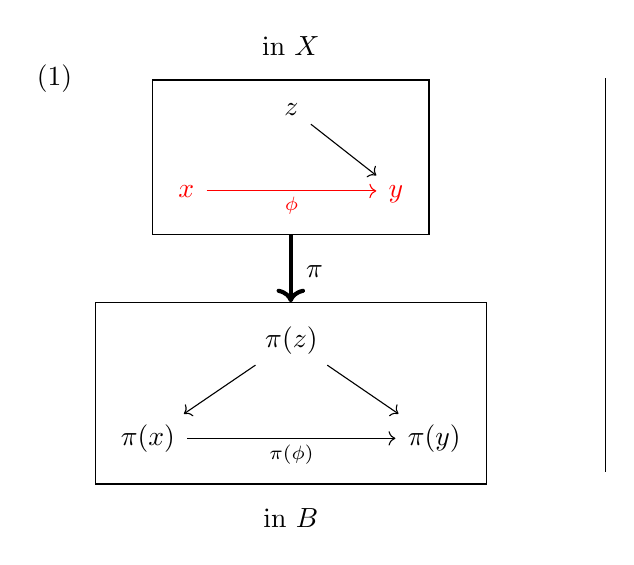
\begin{tikzpicture}[mybox/.style={draw, inner sep=5pt}]
    \node[mybox] (X) at (0,3){%
        \begin{tikzcd}
            {} & z \ar[rd]& {} \\
            \color{red}x \ar[rr, red, "\phi"'] &{}& \color{red}y
        \end{tikzcd}
    };
    \node[mybox] (B) at (0,0){%
        \begin{tikzcd}
            {} & \pi(z) \ar[rd]\ar[ld]& {} \\
            \pi(x) \ar[rr, "\pi(\phi)"'] &{}& \pi(y)
        \end{tikzcd}
    };

    \node [above=5pt of X] {in $\cat{X}$};
    \node [below=5pt of B] {in $\cat{B}$};
    \draw [->, line width=1.5pt] (X) edge (B);
    \node at (0.3,1.55) {$\pi$};
    \draw (4,4) -- (4,-1);
    \node at (-3,4) {($1$)};
    \end{tikzpicture}
    \qquad \qquad
    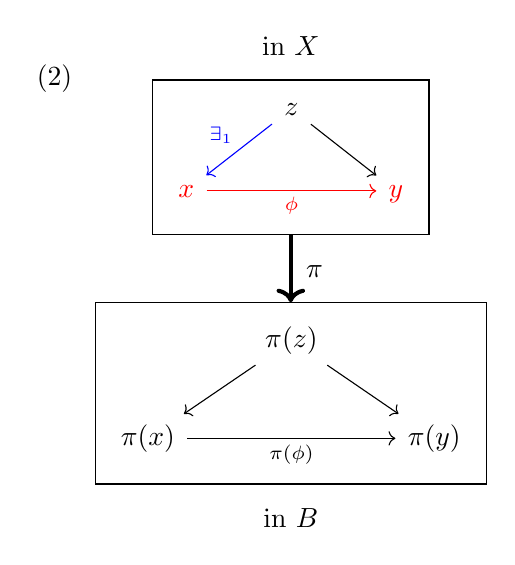
\begin{tikzpicture}[mybox/.style={draw, inner sep=5pt}]
    \node[mybox] (X) at (0,3){%
        \begin{tikzcd}
            {} & z \ar[rd] \ar[ld, blue, "\exists_1"']& {} \\
            \color{red}x \ar[rr, red, "\phi"'] &{}& \color{red}y
        \end{tikzcd}
    };
    \node[mybox] (B) at (0,0){%
        \begin{tikzcd}
            {} & \pi(z) \ar[rd]\ar[ld]& {} \\
            \pi(x) \ar[rr, "\pi(\phi)"'] &{}& \pi(y)
        \end{tikzcd}
    };

    \node [above=5pt of X] {in $\cat{X}$};
    \node [below=5pt of B] {in $\cat{B}$};
    \draw [->, line width=1.5pt] (X) edge (B);
    \node at (0.3,1.55) {$\pi$};
    \node at (-3,4) {($2$)};
    \end{tikzpicture}
    \end{center}
    \end{table}
    %% }}}

\item
    次の性質(Arrow Liftingという)をもつ
    $\pi \colon \cat{X} \to \cat{B}$をfibered categoryという:
    $y \in \cat{X}, u \to \pi(y) \in \cat{B}$が存在する時,
    \underline{$x \in \cat{X}$とcartesian arrow :: $x \to y \in \cat{X}$が存在し},
    以下の図式を満たす
    \footnote{すなわち,$\pi(x)=u, \pi(x \to y)=u \to \pi(y)$を満たす.}.
    \begin{center}
    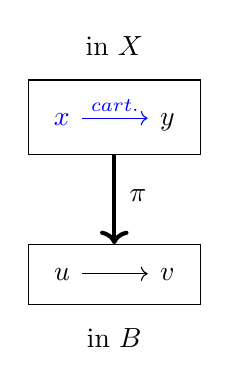
\begin{tikzpicture}[mybox/.style={draw, inner sep=5pt}]
    \node[mybox] (X) at (0,2){%
    \begin{tikzcd}
        \color{blue}x \ar[r, blue, "\text{cart.}"]& y
    \end{tikzcd}
    };
    \node[mybox] (B) at (0,0){%
    \begin{tikzcd}
        u \ar[r]& v
    \end{tikzcd}
    };

    \node [above=5pt of X] {in $\cat{X}$};
    \node [below=5pt of B] {in $\cat{B}$};
    \draw [->, line width=1.5pt] (X) edge (B);
    \node at (0.3,1) {$\pi$};
    \end{tikzpicture}
    \end{center}

\item
    二つのfibered category :: 
    $\pi \colon \cat{X} \to \cat{B}, \pi' \colon \cat{X}' \to \cat{B}$について,
    $\cat{X}$と$\cat{X}'$の間の射とは,
    functor :: $g \colon \cat{X} \to \cat{X}'$であって,
    $\pi, \pi'$と整合的\footnote{ すなわち$\pi' \circ g=\pi$を満たす. }であり,
    cartesian arrowをcartesian arrowに写すもの.

\item
    二つのfibered category :: 
    $\pi \colon \cat{X} \to \cat{B}, \pi' \colon \cat{X}' \to \cat{B}$の間の$2$つの射
    $g,g' \colon \cat{X} \to \cat{X}'$と
    natural transformation :: $\alpha \colon g \to g'$を考える.
    \begin{center}
    \begin{tikzcd}[column sep=3cm]
        \cat{X} \ar[rd, "\pi"]\ar[dd, shift right=3mm, "g"'{name=g}] \ar[dd, shift left=3mm, "g'"{name=gg}]& {} \\
        {} & \cat{B} \\
        \cat{X}' \ar[ru, "\pi'"']& {}
        \ar[Rightarrow, from=g, to=gg, "\alpha"]
    \end{tikzcd}
    \end{center}
    任意の$x \in \cat{X}$について,
    $\pi'(\alpha_x) \colon \pi'(g(x)) \to \pi'(g'(x))$が恒等射になるとき,
    $\alpha$をbase-preserving natural transformationという.
\end{myenum}
\end{Def}

\begin{Remark}
    ここで定義した性質を階層別にまとめると次のように成る.
    \begin{center}
    \begin{tabular}{lcl|l}
        \hline
        $1$-morphism &=& $1$-cell, arrow & (i) Cartesian Arrow, (ii) Arrow Lifting \\ \hline
        $2$-morphism &=& $2$-cell, functor & (iii) Morphism of Fibered Category \\ \hline
        $3$-morphism &=& $3$-cell, natural transformation & (iv) Base-Preserving Natural Transformation \\
        \hline
    \end{tabular}
    \end{center}
    なお,圏の対象(object)はしばしば$0$-cell,圏の射は$1$-cell,等々と呼ばれる.
\end{Remark}

\begin{Remark}
    少し圏論の言葉を整理しておく.
    通常の圏の対象のisoを$1$-isoと呼び$\kiso[1]$と書く.
    この時,階層ごとのiso/equivは以下のようなものである.
    \begin{center}
        \begin{tabular}{lccl}
            $1$-iso. & $x \kiso[1] y$& $\iff$ &
                $2$つの$1$-morphism $\phi \colon x \rightleftarrows y \colon \psi$が存在し, 
                $\psi \circ \phi=\id[x], \phi \circ \psi=\id[y]$.\\ \hline
            $2$-iso. & $x \kiso[2] y$& $\iff$ &
                $2$つの$2$-morphism $\phi \colon x \rightleftarrows y \colon \psi$が存在し, 
                $\psi \circ \phi=\id[x], \phi \circ \psi=\id[y]$.\\
            $2$-equiv. & $x \kequiv[2] y$& $\iff$ &
                $2$つの$2$-morphism $\phi \colon x \rightleftarrows y \colon \psi$が存在し, 
                $\psi \circ \phi \kiso[1] \id[x], \phi \circ \psi \kiso[1] \id[y]$.\\ \hline
            $3$-iso. & $x \kiso[3] y$& $\iff$ &
                $2$つの$3$-morphism $\phi \colon x \rightleftarrows y \colon \psi$が存在し, 
                $\psi \circ \phi=\id[x], \phi \circ \psi=\id[y]$.\\
            $3$-equiv. & $x \kequiv[3] y$& $\iff$ &
                $2$つの$3$-morphism $\phi \colon x \rightleftarrows y \colon \psi$が存在し, 
                $\psi \circ \phi \kiso[2] \id[x], \phi \circ \psi \kiso[2] \id[y]$.\\
        \end{tabular}
    \end{center}
\end{Remark}

\begin{Def}[Fibered Category]
\begin{myenum}
\item
    fibered category over $\cat{B}$が成す圏を$\Fib_{\cat{B}}$とする.
\item
    $\Fib_{\cat{B}}$の部分圏で,
    $2$-morphism(natural transformation)がbase-preserving natural transformationに限られる圏を
    $\FibBP_{\cat{B}}$と書く.
\end{myenum}
\end{Def}

\begin{Remark}
    $\Fib_{\cat{B}}, \FibBP_{\cat{B}}$は$2$-categoryである.
    $2$-categoryは$2$-morphism ($\Fib_{\cat{B}}$ではnatural transformation)に
    ``vertical composition"と``horizontal composition"の二種類の合成が定まる圏である.
    詳しくはこのノートでは触れない.
\end{Remark}

\begin{Def}[Equivalence, $\HOM$]
\begin{myenum}
\item
    $\FibBP_{\cat{B}}$における$2$-equivalenceを単に
    equivalence of morphism of fibered categories over $\cat{B}$と呼ぶ.
\item
    $\cat{X}, \cat{Y} \in \Fib_{\cat{B}}$について
    \[ \HOM_{\cat{B}}(\cat{X}, \cat{Y}):=\Hom_{\FibBP_{\cat{B}}}(\cat{X}, \cat{Y}) \]
    と略す.
\end{myenum}
\end{Def}

\section{Examples : Fibered Categories}
schemes over a scheme
$\Sch/X \to \Sch$

\section{Propositions : Fibered Categories}
2-Yoneda Lemma
``a version of the Yoneda lemma for fibered categories,"
``fully faithfull/equivalence iff fiber locally so"

\section{Definition : Fiber of Fibered Categories}
\begin{Def}[Fiber]
\end{Def}
\begin{Remark}
    $B$-rational point
    $2$-Yoneda Lemma
\end{Remark}

\section{Proposition : Fiber of Fibered Categories}

\section{Motivation : Category Fibered in Groupoids/Sets}

\section{Definition : Category Fibered in Groupoids/Sets}
\begin{Def}[Groupoid, Category fibered in groupoids/sets]
\end{Def}

\begin{Def}[Category fibered in groupoid (Another Definition)]
\end{Def}

\section{Propositions : Category Fibered in Groupoids/Sets}

\bibliographystyle{jplain}
\bibliography{reference}
\end{document}
